\documentclass{article}
\usepackage[parfill]{parskip}
\usepackage[a4paper, total={6in, 9in}]{geometry}

\usepackage{titlesec}
\titlespacing*{\section}{0pt}{0.01\baselineskip}{0.01\baselineskip}

\usepackage{graphicx} %Paquete para incluir imagenes

\titleformat{\paragraph}
{\normalfont\normalsize\bfseries}{\theparagraph}{1em}{}
\titlespacing*{\paragraph}
{0pt}{3.25ex plus 1ex minus .2ex}{1.5ex plus .2ex}


\graphicspath{ {./images/} }
%\usepackage[margin=1cm]{geometry} % Centra el texto

\begin{document}

\begin{titlepage}
  \vspace*{1cm}

  \begin{center}
    {\Huge{Informe del Trabajo Practico 1}}
  \end{center}

  \vspace{0.4cm}

  \begin{center}
    {\LARGE{Facultad de Ingeniería de la Universidad de Buenos Aires}}\\
    \vspace{0.3cm}
  \end{center}

  \vspace{0.8cm}
  \begin{center}
    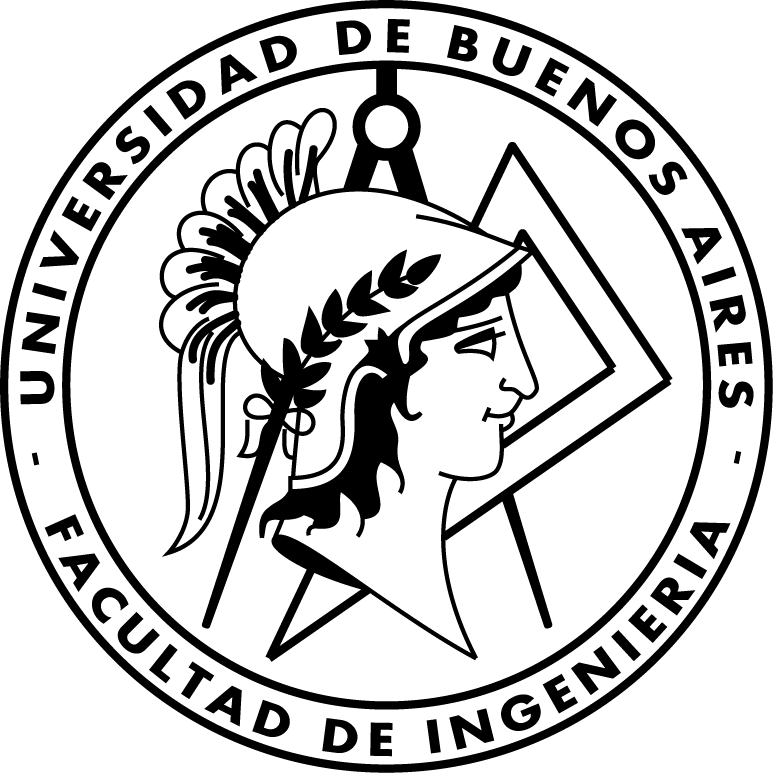
\includegraphics[scale=0.8]{Logo-fiuba}
  \end{center}

  \vspace{0.4cm}
  \begin{center}
    {\Large{Grupo 09}}\\
    \vspace{0.6cm}
    {\begin{minipage}[t]{.32\textwidth}
        \begin{center}
	Castro  Martinez, Jose Ignacio\\
          {\small{Padrón: 106957}}\\
          {\small{email: jacastrom@fi.uba.ar}}
        \end{center}
	\end{minipage}
	\begin{minipage}[t]{.32\textwidth}
        \begin{center}
	Douce, German Alejandro\\
          {\small{Padrón: 106001}}\\
          {\small{email: gdouce@fi.uba.ar}}\\
        \end{center}
      \end{minipage}
      \begin{minipage}[t]{.32\textwidth}
        \begin{center}
          Orsi, Tomas Fabrizio\\
          {\small{Padrón: 109735}}\\
          {\small{email: torsi@fi.uba.ar}}
        \end{center}
      \end{minipage}}
  \end{center}
\end{titlepage}

\section*{Reporte final}
En este trabajo, se consiguió estudiar, analizar y construir diversos modelos que permitieron llevar a cabo la tarea de predecir, con una seguridad relativamente alta, el valor de una variable basado en el estudio de un conjunto de datos. Particularmente, la cancelación de una reserva de hotel.
El trabajo estuvo dividido en las siguientes 4 partes:
\begin{itemize}
	\item Análisis Exploratorio + Ingeniería de Features
	\item Árboles de decisión
	\item Knn, SVM  y Ensamble de modelos
	\begin{itemize}
		\item KNN
		\item SVM
		\item Random Forest
		\item XGBoost
		\item Voting
		\item Stacking
	\end{itemize}
	\item Redes neuronales.
\end{itemize}

En la primera entrega se realizó un primer acercamiento a los datos con los que trabajamos. Graficamos las variables para ver su comportamiento y características generales y utilizamos métodos univariados y multivariados para la detección y tratamiento de outliers tales como z-score, gráficos en 2D y 3D, imputación de valores por la media y eliminación de entradas. De esta forma buscamos tener un dataset lo más limpio posible para obtener la máxima precisión y efectividad al predecir con los modelos. 
Previo a la construcción y predicción realizada con los modelos debimos homologar los datasets de entrenamiento y testeo. Lo cual implicó, aplicarle al dataset de testeo las modificaciones realizadas sobre las columnas del dataset de entrenamiento.

En las siguientes etapas se construyeron varios modelos para realizar una predicción sobre los datos. Todos con características muy variadas, de manera que, se pueda detectar cual de ellos es el que mejor se adapta a la hora de realizar una predicción sobre los datos previamente tratados.

Para medir la precisión y capacidad de generalización del modelo utilizamos la métrica F1 debido a que tiene en cuenta tanto el recall como la precisión. El modelo con el que obtuvimos el mejor valor de esta métrica fue XGBoost con un valor de 0,8423 en la competencia de Kaggle seguido por voting que dio prácticamente lo mismo (0,84007) y Random Forest que dio 0,819. 
En el caso de los clasificadores SVM Y KNN no se obtuvieron muy buenos resultados (0,60 y 0,76 respectivamente).

Finalmente, la red neuronal construida nos dio valores de la métrica F1 muy inferiores a los otros modelos (0.67 en este caso)  
Por otro lado, se confirma una observación anteriormente planteada en la cual, se consideraba mejor a los modelos basados en árboles de decisión. A pesar de que la gran mayoría de los modelos consiguen tener buenas métricas luego de haber sido optimizado por hiperparametros. 

Como detalle final, pudimos observar que, a pesar de su fama, las redes neuronales no implicaron una mejora sustancial en comparación con los otros algoritmos. A pesar, de que estas últimas requirieron una complejidad computacional mucho mayor. 


\end{document}
